\documentclass{report}

\usepackage{amsmath, amssymb}
\usepackage[]{graphicx}
\usepackage[]{color}

%% commands from jss.cls
\newcommand\code{\bgroup\@makeother\_\@makeother\~\@makeother\$\@codex}
\def\@codex#1{{\normalfont\ttfamily\hyphenchar\font=-1 #1}\egroup}
% \let\code=\texttt
\let\proglang=\textsf
\newcommand{\pkg}[1]{{\fontseries{b}\selectfont #1}}
\newcommand{\email}[1]{\href{mailto:#1}{\normalfont\texttt{#1}}}
\newcommand{\E}{\mathsf{E}}
\newcommand{\VAR}{\mathsf{VAR}}
\newcommand{\COV}{\mathsf{COV}}
\newcommand{\Prob}{\mathsf{P}}

\usepackage{bm}
\newcommand{\bb}{\bm{\beta}}
\newcommand{\dif}{\mathrm{d}}
\newcommand{\bg}{\bm{\gamma}}
\newcommand{\bth}{\bm{\theta}}
\newcommand{\bx}{\bm{x}}
\newcommand{\ox}{\overline{x}}
\newcommand{\obx}{\overline{\bm{x}}}

%% maxwidth is the original width if it is less than linewidth
%% otherwise use linewidth (to make sure the graphics do not exceed the margin)
\makeatletter
\def\maxwidth{ %
  \ifdim\Gin@nat@width>\linewidth
    \linewidth
  \else
    \Gin@nat@width
  \fi
}
\makeatother

\definecolor{fgcolor}{rgb}{0.345, 0.345, 0.345}
\newcommand{\hlnum}[1]{\textcolor[rgb]{0.686,0.059,0.569}{#1}}%
\newcommand{\hlstr}[1]{\textcolor[rgb]{0.192,0.494,0.8}{#1}}%
\newcommand{\hlcom}[1]{\textcolor[rgb]{0.678,0.584,0.686}{\textit{#1}}}%
\newcommand{\hlopt}[1]{\textcolor[rgb]{0,0,0}{#1}}%
\newcommand{\hlstd}[1]{\textcolor[rgb]{0.345,0.345,0.345}{#1}}%
\newcommand{\hlkwa}[1]{\textcolor[rgb]{0.161,0.373,0.58}{\textbf{#1}}}%
\newcommand{\hlkwb}[1]{\textcolor[rgb]{0.69,0.353,0.396}{#1}}%
\newcommand{\hlkwc}[1]{\textcolor[rgb]{0.333,0.667,0.333}{#1}}%
\newcommand{\hlkwd}[1]{\textcolor[rgb]{0.737,0.353,0.396}{\textbf{#1}}}%
\let\hlipl\hlkwb

\usepackage{framed}
\makeatletter
\newenvironment{kframe}{%
 \def\at@end@of@kframe{}%
 \ifinner\ifhmode%
  \def\at@end@of@kframe{\end{minipage}}%
  \begin{minipage}{\columnwidth}%
 \fi\fi%
 \def\FrameCommand##1{\hskip\@totalleftmargin \hskip-\fboxsep
 \colorbox{shadecolor}{##1}\hskip-\fboxsep
     % There is no \\@totalrightmargin, so:
     \hskip-\linewidth \hskip-\@totalleftmargin \hskip\columnwidth}%
 \MakeFramed {\advance\hsize-\width
   \@totalleftmargin\z@ \linewidth\hsize
   \@setminipage}}%
 {\par\unskip\endMakeFramed%
 \at@end@of@kframe}
\makeatother

\definecolor{shadecolor}{rgb}{.97, .97, .97}
\definecolor{messagecolor}{rgb}{0, 0, 0}
\definecolor{warningcolor}{rgb}{1, 0, 1}
\definecolor{errorcolor}{rgb}{1, 0, 0}
\newenvironment{knitrout}{}{} % an empty environment to be redefined in TeX

% added for using R markdown
\usepackage{fancyvrb}
\newcommand{\VerbBar}{|}
\newcommand{\VERB}{\Verb[commandchars=\\\{\}]}
\DefineVerbatimEnvironment{Highlighting}{Verbatim}{commandchars=\\\{\}}
% Add ',fontsize=\small' for more characters per line
\usepackage{framed}
\definecolor{shadecolor}{RGB}{248,248,248}
\newenvironment{Shaded}{\begin{snugshade}}{\end{snugshade}}
\newcommand{\AlertTok}[1]{\textcolor[rgb]{0.94,0.16,0.16}{#1}}
\newcommand{\AnnotationTok}[1]{\textcolor[rgb]{0.56,0.35,0.01}{\textbf{\textit{#1}}}}
\newcommand{\AttributeTok}[1]{\textcolor[rgb]{0.77,0.63,0.00}{#1}}
\newcommand{\BaseNTok}[1]{\textcolor[rgb]{0.00,0.00,0.81}{#1}}
\newcommand{\BuiltInTok}[1]{#1}
\newcommand{\CharTok}[1]{\textcolor[rgb]{0.31,0.60,0.02}{#1}}
\newcommand{\CommentTok}[1]{\textcolor[rgb]{0.56,0.35,0.01}{\textit{#1}}}
\newcommand{\CommentVarTok}[1]{\textcolor[rgb]{0.56,0.35,0.01}{\textbf{\textit{#1}}}}
\newcommand{\ConstantTok}[1]{\textcolor[rgb]{0.00,0.00,0.00}{#1}}
\newcommand{\ControlFlowTok}[1]{\textcolor[rgb]{0.13,0.29,0.53}{\textbf{#1}}}
\newcommand{\DataTypeTok}[1]{\textcolor[rgb]{0.13,0.29,0.53}{#1}}
\newcommand{\DecValTok}[1]{\textcolor[rgb]{0.00,0.00,0.81}{#1}}
\newcommand{\DocumentationTok}[1]{\textcolor[rgb]{0.56,0.35,0.01}{\textbf{\textit{#1}}}}
\newcommand{\ErrorTok}[1]{\textcolor[rgb]{0.64,0.00,0.00}{\textbf{#1}}}
\newcommand{\ExtensionTok}[1]{#1}
\newcommand{\FloatTok}[1]{\textcolor[rgb]{0.00,0.00,0.81}{#1}}
\newcommand{\FunctionTok}[1]{\textcolor[rgb]{0.00,0.00,0.00}{#1}}
\newcommand{\ImportTok}[1]{#1}
\newcommand{\InformationTok}[1]{\textcolor[rgb]{0.56,0.35,0.01}{\textbf{\textit{#1}}}}
\newcommand{\KeywordTok}[1]{\textcolor[rgb]{0.13,0.29,0.53}{\textbf{#1}}}
\newcommand{\NormalTok}[1]{#1}
\newcommand{\OperatorTok}[1]{\textcolor[rgb]{0.81,0.36,0.00}{\textbf{#1}}}
\newcommand{\OtherTok}[1]{\textcolor[rgb]{0.56,0.35,0.01}{#1}}
\newcommand{\PreprocessorTok}[1]{\textcolor[rgb]{0.56,0.35,0.01}{\textit{#1}}}
\newcommand{\RegionMarkerTok}[1]{#1}
\newcommand{\SpecialCharTok}[1]{\textcolor[rgb]{0.00,0.00,0.00}{#1}}
\newcommand{\SpecialStringTok}[1]{\textcolor[rgb]{0.31,0.60,0.02}{#1}}
\newcommand{\StringTok}[1]{\textcolor[rgb]{0.31,0.60,0.02}{#1}}
\newcommand{\VariableTok}[1]{\textcolor[rgb]{0.00,0.00,0.00}{#1}}
\newcommand{\VerbatimStringTok}[1]{\textcolor[rgb]{0.31,0.60,0.02}{#1}}
\newcommand{\WarningTok}[1]{\textcolor[rgb]{0.56,0.35,0.01}{\textbf{\textit{#1}}}}

\usepackage{alltt}
\usepackage{graphicx}
\usepackage[margin=1cm]{geometry}
\usepackage{color}
\usepackage[pages=absolute]{flowfram}
\usepackage{lipsum}
\usepackage{url, pdfpages}
\usepackage{enumitem}
\setlist{itemsep = 0pt, topsep = 1pt, leftmargin = 0.6mm}
\usepackage[anythingbreaks]{breakurl}
\usepackage{microtype}
\usepackage{anyfontsize}
\usepackage{caption}
\usepackage{wrapfig}
\usepackage{scrextend}
\usepackage{booktabs}

% added
\usepackage{natbib}

\renewcommand{\UrlBreaks}{\do\/\do\a\do\b\do\c\do\d\do\e\do\f\do\g\do\h\do\i\do\j\do\k\do\l\do\m\do\n\do\o\do\p\do\q\do\r\do\s\do\t\do\u\do\v\do\w\do\x\do\y\do\z\do\A\do\B\do\C\do\D\do\E\do\F\do\G\do\H\do\I\do\J\do\K\do\L\do\M\do\N\do\O\do\P\do\Q\do\R\do\S\do\T\do\U\do\V\do\W\do\X\do\Y\do\Z}

\usepackage{algorithm, algorithmic}

%% for knitr
\usepackage[unicode=true,pdfusetitle,
 bookmarks=true,bookmarksnumbered=true,bookmarksopen=true,bookmarksopenlevel=2,
 breaklinks=false,pdfborder={0 0 1},backref=false,colorlinks=false]
 {hyperref}
\hypersetup{
 pdfstartview={XYZ null null 1}}

% graph path
\graphicspath{{images/}}
\DeclareGraphicsExtensions{.eps,. ps,. pdf, .jpg, .png}

\twocolumn

\begin{document}


% \section*{Software Review}
\section*{Regularized Cox Cure Rate Model with R package \pkg{intsurv}}

In this column, we demonstrate the usage of the function
\VERB|\KeywordTok{cox\_cure\_net.fit}\NormalTok{()}| provided by
\proglang{R} package \pkg{intsurv} (Wang 2019) for fitting regularized
Cox cure rate model with elastic-net penalty (Zou and Hastie 2005).

The cure rate models first proposed by Berkson and Gage (1952) are
commonly adopted statistical methods for survival data with a cure
fraction. Consider a random sample of \(n\) subjects with
right-censoring data and a cured fraction. Let \(T_j=\min(V_j, C_j)\)
and \(\Delta_j=I(V_j > C_j)\), where \(V_j\) and \(C_j\) represents the
random variable of the event time and the censoring time of subject
\(j\), respectively, \(I(\cdot)\) is indicator function,
\(j\in\{1,\ldots,n\}\). Define \(Z_j = 1\) if subject \(j\) is
susceptible, and \(Z_j = 0\) otherwise, with probability
\(p_j = \Pr(Z_j = 1)\). Notice that \(Z_j\) is observed to be 1 if
\(\Delta_j=1\) and is missing otherwise. Proposed by Farewell (1982), a
logistic model \(p_j=1/[1+\exp(-\gamma_0-\bx^{\top}_j\bg)]\) is widely
used, where \(\bx_j\) represents the covariate vector of subject \(j\)
(excluding intercept), \(\gamma_0\) is unknown coefficient of intercept
and \(\bg\) is a vector of unknown covariate coefficients. Given that
\(Z_j = 1\), Kuk and Chen (1992) proposed modeling the conditional
survival times through a Cox proportional hazard model with the hazard
function
\[h_j(t\mid Z_j = 1) = h_0(t\mid Z_j = 1) \exp(\bx_j^{\top}\bb),\] where
\(h_0(t\mid Z_j = 1)\) is an unspecified baseline function for events,
and \(\bb\) is a vector of unknown coefficients of the covariate vector
\(\bx_j\). The conditional survival function of the event time of
subject \(j\) is
\[S_j(t\mid Z_j = 1) = \exp\{-H_0(t\mid Z_j = 1) \exp(\bx_j^{\top} \bb) \},\]
where \(H_0(t\mid Z_j = 1) = \int_0^t h_0(s\mid Z_j = 1) \dif s\). Given
that subject \(j\) is cured (\(Z_j = 0\)), the conditional survival
function satisfies \(S_j(t\mid Z_j=0) = 1\), for \(t<+\infty\). The
observed data likelihood function can be written as
\begin{align}\label{eqn:mod}
L(\bm{\theta}) = \prod_{j=1}^n
& \left\{ p_j h_j(t_j\mid Z_j=1) S_j(t_j\mid Z_j=1) \right\}^{\delta_j}\nonumber\\
& \left\{(1 - p_j) + p_j S_j(t_j \mid Z_j = 1)\right\}^{1-\delta_j},
\end{align} where \(\bm{\theta}=\{\bb,\bg,\gamma_0,h_0(\cdot)\}\). A
model estimation procedure based on the well-known EM algorithm was
proposed by Sy and Taylor (2000). Recently, a few works have been
proposed to perform variable selection for cure models. For example,
Scolas et al. (2016) proposed variable selection with adaptive lasso
penalty (Zou 2006) for interval-censored data in a parametric cure
model, where conditional survival times follow the extended generalized
gamma distribution. Masud, Tu, and Yu (2018) proposed variable selection
methods for mixture cure model and promotion cure model through
regularization by the adaptive lasso penalty. Fan et al. (2017) and Shi,
Ma, and Huang (2019) promoted structural similarity and sign consistency
of \(\hat{\bg}\) and \(\hat{\bb}\), respectively, with minimax concave
penalty (Zhang 2010) for variable selection. Here, we concentrate on the
following regularized estimator with elastic-net penalty, \begin{align}
  \hat{\bm{\theta}} = \arg\min_{\bm{\theta}} -\frac{1}{n}
  \ell(\bm{\theta})
  + P_{1}(\bb; \alpha_1, \lambda_1) + P_{2}(\bg; \alpha_2, \lambda_2),
\end{align} where \(\ell(\bm{\theta})\) is the log-likelihood function
under the observed data from \eqref{eqn:mod} and \begin{align*}
  P_{1}(\bb; \alpha_1, \lambda_1)
  & = \lambda_1 \left( \alpha_1 \sum_{k=1}^{p} \omega_k \lvert \beta_k \rvert +
  \frac{1 - \alpha_1}{2} \sum_{k=1}^{p} \beta_k^2\right),\\
  P_{2}(\bg; \alpha_2, \lambda_2)
  & = \lambda_2 \left( \alpha_2 \sum_{k=1}^{p} \nu_k \lvert \gamma_k \rvert +
  \frac{1 - \alpha_2}{2} \sum_{k=1}^{p} \gamma_k^2 \right),
\end{align*} where \(\omega_k\) and \(\nu_k\) represent non-negative
weights (Zou 2006), \(0\le\alpha_1\le1\), \(0\le\alpha_2\le1\),
\(\lambda_1\ge0\), and \(\lambda_2\ge0\) are tuning parameters. The
coordinate descent algorithm (Friedman et al. 2007) or local quadratic
approximations (Fan and Li 2001) may be utilized in the M-steps of the
EM algorithm to obtain the regularized estimator. Under the hood,
\VERB|\KeywordTok{cox\_cure\_net.fit}\NormalTok{()}| utilizes the
coordinate-majorization-descent (CMD) algorithm proposed by Yang and Zou
(2013) in the M-steps due to its descent property.

To demonstrate the usage of
\VERB|\KeywordTok{cox\_cure\_net.fit}\NormalTok{()}|, we may simulate a
dataset of sample size 200 as follows. 100 covariates are simulated from
multivariate normal distribution with means zero and variances one. The
correlation between \(x_k\) and \(x_l\), \(k\neq l\), was set to be
\(\rho^{\lvert k - l \rvert}\), where \(\rho = 0.5\). For each model
part, only five covariates actually have non-zero coefficients. The true
non-zero coefficients are simulated from \(\mathrm{Unif}(0.6, 1)\)
independently. For susceptible subjects, the event times were generated
from Weibull-Cox model with baseline hazard function
\(h_0(t; \bx) = 0.2t\exp(\bx^{\top}\bb)\). For cured subjects, the event
times were set to be infinity. The censoring times were generated
independently with the event times from exponential distribution with
rate 0.01 and truncated at 10. The generation of event times and
censoring times takes advantage of function
\VERB|\NormalTok{intsurv}\OperatorTok{::}\KeywordTok{simData4cure}\NormalTok{()}|.

\begin{Shaded}
\begin{Highlighting}[]
\KeywordTok{library}\NormalTok{(intsurv)}
\KeywordTok{set.seed}\NormalTok{(}\DecValTok{123}\NormalTok{)}
\NormalTok{p <{-}}\StringTok{ }\DecValTok{100}\NormalTok{; n <{-}}\StringTok{ }\DecValTok{200}\NormalTok{; rho <{-}}\StringTok{ }\FloatTok{0.5}
\NormalTok{beta0 <{-}}\StringTok{ }\NormalTok{gamma0 <{-}}\StringTok{ }\KeywordTok{rep}\NormalTok{(}\DecValTok{0}\NormalTok{, p)}
\NormalTok{beta0[}\KeywordTok{c}\NormalTok{(}\DecValTok{1}\NormalTok{, }\DecValTok{2}\NormalTok{, }\DecValTok{4}\NormalTok{, }\DecValTok{6}\NormalTok{, }\DecValTok{8}\NormalTok{)] <{-}}\StringTok{ }\KeywordTok{runif}\NormalTok{(}\DecValTok{5}\NormalTok{, }\FloatTok{0.6}\NormalTok{, }\DecValTok{1}\NormalTok{)}
\NormalTok{gamma0[}\KeywordTok{c}\NormalTok{(}\DecValTok{1}\NormalTok{, }\DecValTok{3}\NormalTok{, }\DecValTok{5}\NormalTok{, }\DecValTok{7}\NormalTok{, }\DecValTok{9}\NormalTok{)] <{-}}\StringTok{ }\KeywordTok{runif}\NormalTok{(}\DecValTok{5}\NormalTok{, }\FloatTok{0.6}\NormalTok{, }\DecValTok{1}\NormalTok{)}
\NormalTok{ij\_mat <{-}}\StringTok{ }\KeywordTok{expand.grid}\NormalTok{(}\DataTypeTok{i =} \KeywordTok{seq\_len}\NormalTok{(p), }\DataTypeTok{j =} \KeywordTok{seq\_len}\NormalTok{(p))}
\NormalTok{Sigma <{-}}\StringTok{ }\KeywordTok{matrix}\NormalTok{(}\KeywordTok{mapply}\NormalTok{(}\ControlFlowTok{function}\NormalTok{(i, j) \{}
\NormalTok{    rho}\OperatorTok{\^{}}\KeywordTok{abs}\NormalTok{(i }\OperatorTok{{-}}\StringTok{ }\NormalTok{j)}
\NormalTok{\}, ij\_mat}\OperatorTok{$}\NormalTok{i, ij\_mat}\OperatorTok{$}\NormalTok{j), }\DataTypeTok{nrow =}\NormalTok{ p)}
\NormalTok{x\_mat <{-}}\StringTok{ }\NormalTok{MASS}\OperatorTok{::}\KeywordTok{mvrnorm}\NormalTok{(n, }\DataTypeTok{mu =} \KeywordTok{rep}\NormalTok{(}\DecValTok{0}\NormalTok{, p), Sigma)}
\KeywordTok{colnames}\NormalTok{(x\_mat) <{-}}\StringTok{ }\KeywordTok{paste0}\NormalTok{(}\StringTok{"x"}\NormalTok{, }\KeywordTok{seq\_len}\NormalTok{(p))}
\NormalTok{dat <{-}}\StringTok{ }\KeywordTok{simData4cure}\NormalTok{(}
\NormalTok{    n, }\DataTypeTok{survMat =}\NormalTok{ x\_mat, }\DataTypeTok{survCoef =}\NormalTok{ beta0,}
    \DataTypeTok{cureCoef =}\NormalTok{ gamma0, }\DataTypeTok{b0 =} \DecValTok{1}\NormalTok{, }\DataTypeTok{lambda\_censor =} \FloatTok{0.01}\NormalTok{,}
    \DataTypeTok{max\_censor =} \DecValTok{10}\NormalTok{, }\DataTypeTok{p1 =} \DecValTok{1}\NormalTok{, }\DataTypeTok{p2 =} \DecValTok{1}\NormalTok{, }\DataTypeTok{p3 =} \DecValTok{1}
\NormalTok{)}
\end{Highlighting}
\end{Shaded}

Similar to function
\VERB|\NormalTok{glmnet}\OperatorTok{::}\KeywordTok{glmnet}\NormalTok{()}|
for regularized generalized linear models, \texttt{cox\_cure\_net.fit()}
fits the regularized Cox cure rate model over a specified grid of tuning
parameter \(\lambda_1\) and \(\lambda_2\) with fixed \(\alpha_1\) and
\(\alpha_2\). Instead, the desired length of each \(\lambda\) sequence
can be specified and an equally-spaced (in logarithm scale) sequence
will be generated from the smallest ``large enough'' \(\lambda_{\max}\)
that result in all zero coefficient estimates to a specified ``small
enough'' \(\lambda_{\min}\). By default,
\(\lambda_{\min}=0.1\lambda_{\max}\) is set for both model parts in
\VERB|\KeywordTok{cox\_cure\_net.fit}\NormalTok{()}|. Here we set
\(\alpha_1 = \alpha_2 = 0.5\) and specify a 10 by 10 grid for
\(\lambda_1\) and \(\lambda_2\).

\begin{Shaded}
\begin{Highlighting}[]
\KeywordTok{system.time}\NormalTok{(\{}
\NormalTok{    fit1 <{-}}\StringTok{ }\KeywordTok{cox\_cure\_net.fit}\NormalTok{(}
        \DataTypeTok{surv\_x =}\NormalTok{ x\_mat, }\DataTypeTok{cure\_x =}\NormalTok{ x\_mat,}
        \DataTypeTok{time =}\NormalTok{ dat}\OperatorTok{$}\NormalTok{obs\_time, }\DataTypeTok{event =}\NormalTok{ dat}\OperatorTok{$}\NormalTok{obs\_event,}
        \DataTypeTok{surv\_nlambda =} \DecValTok{10}\NormalTok{, }\DataTypeTok{cure\_nlambda =} \DecValTok{10}\NormalTok{,}
        \DataTypeTok{surv\_alpha =} \FloatTok{0.5}\NormalTok{, }\DataTypeTok{cure\_alpha =} \FloatTok{0.5}
\NormalTok{    )}
\NormalTok{\})}
\end{Highlighting}
\end{Shaded}

\begin{verbatim}
##    user  system elapsed 
##  89.321   0.704  11.320
\end{verbatim}

The tuning parameters may be selected based on BIC and a
\VERB|\KeywordTok{coef}\NormalTok{()}| method for
\VERB|\NormalTok{cox\_cure\_net}| objects can be used to return the
coefficient estimates from the selected model. We may quickly check the
true positive rate and false positive rate in terms of variable
selection as follows:

\begin{Shaded}
\begin{Highlighting}[]
\NormalTok{eval\_vs <{-}}\StringTok{ }\ControlFlowTok{function}\NormalTok{(x, beta0, gamma0) \{}
\NormalTok{    foo <{-}}\StringTok{ }\ControlFlowTok{function}\NormalTok{(b, b0) \{}
        \KeywordTok{c}\NormalTok{(}\StringTok{"\% True Positive"}\NormalTok{ =}\StringTok{ }\KeywordTok{mean}\NormalTok{(b[b0 }\OperatorTok{!=}\StringTok{ }\DecValTok{0}\NormalTok{] }\OperatorTok{!=}\StringTok{ }\DecValTok{0}\NormalTok{),}
          \StringTok{"\% False Positive"}\NormalTok{ =}\StringTok{ }\KeywordTok{mean}\NormalTok{(b[b0 }\OperatorTok{==}\StringTok{ }\DecValTok{0}\NormalTok{] }\OperatorTok{!=}\StringTok{ }\DecValTok{0}\NormalTok{))}
\NormalTok{    \}}
    \KeywordTok{rbind}\NormalTok{(}\DataTypeTok{beta =} \KeywordTok{foo}\NormalTok{(}\KeywordTok{coef}\NormalTok{(fit1)}\OperatorTok{$}\NormalTok{surv, beta0),}
          \DataTypeTok{gamma =} \KeywordTok{foo}\NormalTok{(}\KeywordTok{coef}\NormalTok{(fit1)}\OperatorTok{$}\NormalTok{cure, gamma0))}
\NormalTok{\}}
\KeywordTok{eval\_vs}\NormalTok{(fit1, beta0, gamma0)}
\end{Highlighting}
\end{Shaded}

\begin{verbatim}
##       % True Positive % False Positive
## beta        1.0000000       0.09473684
## gamma       0.8333333       0.07368421
\end{verbatim}

To reduce computational burden, the generalized EM algorithm may be used
by setting one-step CMD update as follows. In this example, we are able
to decrease the computation time by about 80\% and obtain the same
variable selection results.

\begin{Shaded}
\begin{Highlighting}[]
\KeywordTok{system.time}\NormalTok{(\{}
\NormalTok{    fit2 <{-}}\StringTok{ }\KeywordTok{cox\_cure\_net.fit}\NormalTok{(}
        \DataTypeTok{surv\_x =}\NormalTok{ x\_mat, }\DataTypeTok{cure\_x =}\NormalTok{ x\_mat,}
        \DataTypeTok{time =}\NormalTok{ dat}\OperatorTok{$}\NormalTok{obs\_time, }\DataTypeTok{event =}\NormalTok{ dat}\OperatorTok{$}\NormalTok{obs\_event,}
        \DataTypeTok{surv\_nlambda =} \DecValTok{10}\NormalTok{, }\DataTypeTok{cure\_nlambda =} \DecValTok{10}\NormalTok{,}
        \DataTypeTok{surv\_alpha =} \FloatTok{0.5}\NormalTok{, }\DataTypeTok{cure\_alpha =} \FloatTok{0.5}\NormalTok{,}
        \DataTypeTok{surv\_max\_iter =} \DecValTok{1}\NormalTok{, }\DataTypeTok{cure\_max\_iter =} \DecValTok{1}
\NormalTok{    )}
\NormalTok{\})}
\end{Highlighting}
\end{Shaded}

\begin{verbatim}
##    user  system elapsed 
##  18.064   0.135   2.294
\end{verbatim}

\begin{Shaded}
\begin{Highlighting}[]
\KeywordTok{eval\_vs}\NormalTok{(fit2, beta0, gamma0)}
\end{Highlighting}
\end{Shaded}

\begin{verbatim}
##       % True Positive % False Positive
## beta        1.0000000       0.09473684
## gamma       0.8333333       0.07368421
\end{verbatim}

After variable selection, a regular Cox cure rate model may be fitted by
\texttt{intsurv::cox\_cure()}. See \url{https://wenjie-stat.me/intsurv/}
for full package documents.

\section*{Reference}
\setlength{\parindent}{0em}
\setlength{\parskip}{0.15em}

\hypertarget{refs}{}
\leavevmode\hypertarget{ref-berkson1952jasa}{}%
Berkson, Joseph, and Robert P. Gage. 1952. ``Survival Curve for Cancer
Patients Following Treatment.'' \emph{Journal of the American
Statistical Association} 47 (259): 501--15.

\leavevmode\hypertarget{ref-fanLi2001jasa}{}%
Fan, Jianqing, and Runze Li. 2001. ``Variable Selection via Nonconcave
Penalized Likelihood and Its Oracle Properties.'' \emph{Journal of the
American Statistical Association} 96 (456): 1348--60.

\leavevmode\hypertarget{ref-fan2017smmr}{}%
Fan, Xinyan, Mengque Liu, Kuangnan Fang, Yuan Huang, and Shuangge Ma.
2017. ``Promoting Structural Effects of Covariates in the Cure Rate
Model with Penalization.'' \emph{Statistical Methods in Medical
Research} 26 (5): 2078--92.

\leavevmode\hypertarget{ref-farewell1982biometrics}{}%
Farewell, Vern T. 1982. ``The Use of Mixture Models for the Analysis of
Survival Data with Long-Term Survivors.'' \emph{Biometrics}, 1041--6.

\leavevmode\hypertarget{ref-friedman2007aoas}{}%
Friedman, Jerome, Trevor Hastie, Holger Höfling, and Robert Tibshirani.
2007. ``Pathwise Coordinate Optimization.'' \emph{The Annals of Applied
Statistics} 1 (2): 302--32.

\leavevmode\hypertarget{ref-kuk1992biometrika}{}%
Kuk, Anthony Y. C., and Chen-Hsin Chen. 1992. ``A Mixture Model
Combining Logistic Regression with Proportional Hazards Regression.''
\emph{Biometrika} 79 (3): 531--41.

\leavevmode\hypertarget{ref-masud2018smimr}{}%
Masud, Abdullah, Wanzhu Tu, and Zhangsheng Yu. 2018. ``Variable
Selection for Mixture and Promotion Time Cure Rate Models.''
\emph{Statistical Methods in Medical Research} 27 (7): 2185--99.

\leavevmode\hypertarget{ref-scolas2016sim}{}%
Scolas, Sylvie, Anouar El Ghouch, Catherine Legrand, and Abderrahim
Oulhaj. 2016. ``Variable Selection in a Flexible Parametric Mixture Cure
Model with Interval-Censored Data.'' \emph{Statistics in Medicine} 35
(7): 1210--25.

\leavevmode\hypertarget{ref-shi2019smmr}{}%
Shi, Xingjie, Shuangge Ma, and Yuan Huang. 2019. ``Promoting Sign
Consistency in the Cure Model Estimation and Selection.''
\emph{Statistical Methods in Medical Research}, 1--14.

\leavevmode\hypertarget{ref-sy2000biometrics}{}%
Sy, Judy P., and Jeremy M. G. Taylor. 2000. ``Estimation in a Cox
Proportional Hazards Cure Model.'' \emph{Biometrics} 56 (1): 227--36.

\leavevmode\hypertarget{ref-intsurv-package}{}%
Wang, Wenjie. 2019. \emph{intsurv: Integrative Survival Models}.
\url{https://github.com/wenjie2wang/intsurv}.

\leavevmode\hypertarget{ref-yang2013sii}{}%
Yang, Yi, and Hui Zou. 2013. ``A Cocktail Algorithm for Solving the
Elastic Net Penalized Cox's Regression in High Dimensions.''
\emph{Statistics and Its Interface} 6 (2): 167--73.

\leavevmode\hypertarget{ref-zhang2010aos}{}%
Zhang, Cun-Hui. 2010. ``Nearly Unbiased Variable Selection Under Minimax
Concave Penalty.'' \emph{The Annals of Statistics} 38 (2): 894--942.

\leavevmode\hypertarget{ref-zou2006jasa}{}%
Zou, Hui. 2006. ``The Adaptive Lasso and Its Oracle Properties.''
\emph{Journal of the American Statistical Association} 101 (476):
1418--29.

\leavevmode\hypertarget{ref-zouHastie2005jrssb}{}%
Zou, Hui, and Trevor Hastie. 2005. ``Regularization and Variable
Selection via the Elastic Net.'' \emph{Journal of the Royal Statistical
Society: Series B (Statistical Methodology)} 67 (2): 301--20.


\renewcommand{\bibsection}{\section*{Reference}}
\setlength{\bibhang}{0pt}
\setlength{\bibsep}{0.4em}
\bibliographystyle{asa}
\bibliography{cox-cure-net}

\medskip

\noindent
\begin{minipage}[b]{1.2in}\centering
  \sbox0{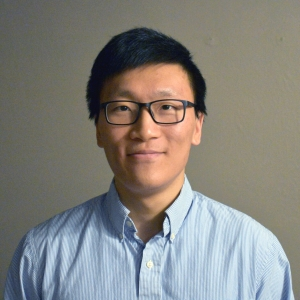
\includegraphics{WenjieWang}}%
  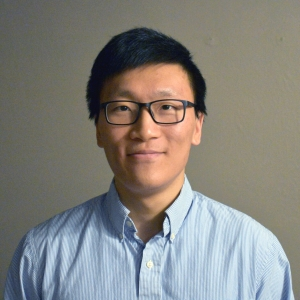
\includegraphics[width=1.2in, trim={{0.08\wd0} {0.08\ht0} {0.08\wd0}
    {0.08\ht0}}, clip=true]{WenjieWang}\\
\end{minipage}
\hspace{0.2cm}
\begin{minipage}[b]{2.4in}
\begin{flushright}
  \emph{Wenjie Wang}\\
  Research Scientist\\
  Machine Learning, Artificial Intelligence, and Connected Care\\
  Advanced Analytics and Data Sciences\\
  Eli Lilly and Company\\
  Email: \email{wang\_wenjie@lilly.com}
\end{flushright}
\end{minipage}


\end{document}
